% -*-cap2.tex-*-
% Este fichero es parte de la plantilla LaTeX para
% la realización de Proyectos Final de Carrera, protegido
% bajo los términos de la licencia GFDL.
% Para más información, la licencia completa viene incluida en el
% fichero fdl-1.3.tex

% Copyright (C) 2009 Pablo Recio Quijano 

\section{Introducción}

El primer paso que vamos a dar para describir el diseño de la aplicación será describir los requisitos del
sistema necesarios para poder ejecutar la aplicación, y posteriormente comentaremos las herramientas que se
van a usar para el desarrollo de la aplicación.

\section{Definición de los requisitos del sistema}

Los requisitos hardware y software necesarios para poder ejecutar con soltura la aplicación son los siguientes:

\begin{itemize}
	\item Sistema operativo Microsoft Windows en su versión Windows 7, o sistemas basados en GNU/Linux tales como
		la distribución Ubuntu en su versión 10.04.
	\item Últimas actualizaciones del sistema instaladas, drivers y demás aplicaciones propias del sistema
		configuradas correctamente.
	\item Procesador igual o superior a 1,6 GHz.
	\item Memoria RAM igual o superior a 512 MB
	\item Tarjeta gráfica con aceleración 3D con un mínimo de 128 MB
	\item En versiones basadas en Linux, se requieren las siguientes librerías:
		\begin{itemize}
			\item python-pygame
			\item python-setuptools
			\item PyOpenGL
			\item PyOpenGL-accelerate
		\end{itemize}
	\item Por otro lado, si el sistema está basado en Microsoft Windows, necesitaremos:
		\begin{itemize}
			\item Pygame
			\item Python OpenGL and Gloss
		\end{itemize}
\end{itemize}

\section{Herramientas utilizadas}

\subsection{Librería gráfica}

Para todo el tema del aspecto gráfico, mi tutor me recomendó que utilizara las librerías SDL\footnote{Simple
Directmedia Layer}, ya que son unas librerías orientadas al desarrollo de videojuegos con varias particularidades:
\begin{itemize}
    \item Son completas, ya que permiten gestionar operaciones de dibujo en dos dimensiones, efectos de
            sonido y música, carga y gestión de imágenes, subsistemas de control de métodos de entrada,
            etcétera, por lo que contamos con una solución global para desarrollar videojuegos.
    \item Están programas en C, por lo que se puede esperar un buen rendimiento de las librerías en
            diferentes entornos.
    \item Multiplataforma: es compatible oficialmente con los sistemas Microsoft Windows, GNU/Linux,
            Mac OS y QNX, además de otras arquitecturas y sistemas menos comunes como Sega Dreamcast, Sony PSP,
            WebOS, Google Android o Symbian entre otros.
    \item Tampoco hay que mantener al margen la característica de que cuenta con wrappers a otros lenguajes
            de programación como entre los que se encuentran C++, Ada, C\#, BASIC, Erlang, Lua, Java o Python, por
            lo que nos da bastante libertad para elegir un lenguaje de programación principal
    \item Publicado bajo licencia LGPL, con todas las ventajas que conlleva.
    \item Y por último no hay que menospreciar que mi tutor emplea SDL a la hora de impartir la asignatura
            de diseño de videojuegos, y contar con esa base de conocimiento nos ayudará a desarrollar más rápidamente
            y solucionar antes nuestros posible problemas.
\end{itemize}

\begin{figure}[h]
  \label{logo-sdl}
  \begin{center}
    
\includegraphics[scale=0.5]{SDL.png}
  \end{center}
  \caption{Logotipo de la librería Simple DirectMedia Layer}
\end{figure}

En este aspecto, la utilización de las librerías SDL estaba clara. Potencia, comodidad, multiplataforma y con la posibilidad
de utilizar diferentes lenguajes de programación.\\

\subsection{Lenguaje de programación}

Una vez que tocamos el tema de los lenguajes de programación, entra en escena la problemática sobre qué lenguaje
utilizar. En principio se pensó emplear el lenguaje C++ por dos sencillas razones:

\begin{enumerate}
    \item Por un lado es un lenguaje que hemos aprendido en la carrera, se ha utilizado en varias asignaturas de
            diferentes ramas, con lo cual la comodidad y familiaridad que podemos tener a la hora de programar
            es un punto importante a tener en cuenta.
    \item Tampoco podemos olvidar que, al ser un lenguaje compilado, la velocidad de ejecución que se consigue
            es interesante, y mucho más tratándose de temas como la inteligencia artificial (donde puede ser
            necesario un uso intensivo de los recursos del sistema) o el desarrollo de videojuegos (en el que
            la potencia del ordenador repercute en una mejor experiencia del usuario)
\end{enumerate}

Pero hay que detenerse un momento y pensar en la naturaleza del proyecto. Aunque el programa a desarrollar sea un
videojuego, no hay que olvidar que hay diferentes tipos de juegos, que pueden condicionar o influir en nuestra forma
de programarlo. En el caso del dominó, lo primero que debemos tener en cuenta es que el apartado gráfico no va a
requerir de una gran potencia o despliegue de efectos: el dominó es un juego pausado y a diferencia de otros
videojuegos lo importante en este caso es mostrar al usuario la información de la partida de una forma clara y sencilla,
para que el jugador evalúe las posibilidades de acción y actúe en consecuencia.\\

\begin{figure}[h]
  \label{logo-python}
  \begin{center}
    
\includegraphics[scale=0.3]{python.png}
  \end{center}
  \caption{Logotipo de Python - Copyright Python Software Foundation}
\end{figure}


Si tenemos en cuenta estas circunstancias, existen otros lenguajes que también deben entrar en juego,
como por ejemplo \textbf{Python}. Buscando las diferencias, ventajas y desventajas de Python frente a C++,
obtenemos el siguiente listado:

\begin{enumerate}
    \item Python es un lenguaje de programación multiparadigma ya que soporta orientación a objetos,
            programación imperativa y, en menor medida, programación funcional.
    \item Al igual que C++ es multiplataforma, y está publicado con la licencia \textbf{Python Software Foundation
            License}, que es una licencia de software libre permisiva, compatible con la GPL.
    \item La sintaxis de Python es muy clara, simple, expresiva y legible, con lo cual los programas
            desarrollados bajo Python son más sencillos de entender \cite{Pilgrim:2004:DP:983200}.
    \item Python es un lenguaje interpretado, a diferencia de C++ que es compilado. Este aspecto podría suponer una
            desventaja ya que al ser interpretado puede resultar más lento, pero analicemos pausadamente estos
            factores:
        \begin{itemize}
            \item Como ya hemos comentado previamente, nuestra aplicación, a pesar de enmarcarse dentro de las
                    facciones de un videojuego, no requiere de grandes alardes de potencia gráfica como podría
                    suponerse, ya que es un tipo de juego pausado y donde cómo se muestra la información
                    es mucho más importante que la velocidad o los efectos de vídeo e imágenes.
            \item A pesar de ser interpretado, un gran conjunto de las funcionalidades de python --- como librerías o
                    funciones básicas del lenguaje --- están programadas internamente en C, así que podríamos
                    verlo como que estamos utilizando la comodidad de Python sobre la potencia de C, uniendo
                    lo mejor de ambos mundos.
        \end{itemize}
\end{enumerate}

\subsection{Diseño y estilo visual de interfaces}

El diseño visual que se ha desarrollado para la interfaz se ha creado desde cero, buscando los siguientes objetivos:
\begin{itemize}
    \item Líneas sencillas, minimalistas, sin recargar innecesariamente la pantalla
    \item Botones grandes, para que sea fácil de utilizar por usuarios de edad avanzada.
    \item Textos con un punto de letra elevado, facilitando la rápida lectura y legibilidad del texto.
\end{itemize}

\begin{figure}[h]
  \label{interfaz}
  \begin{center}
    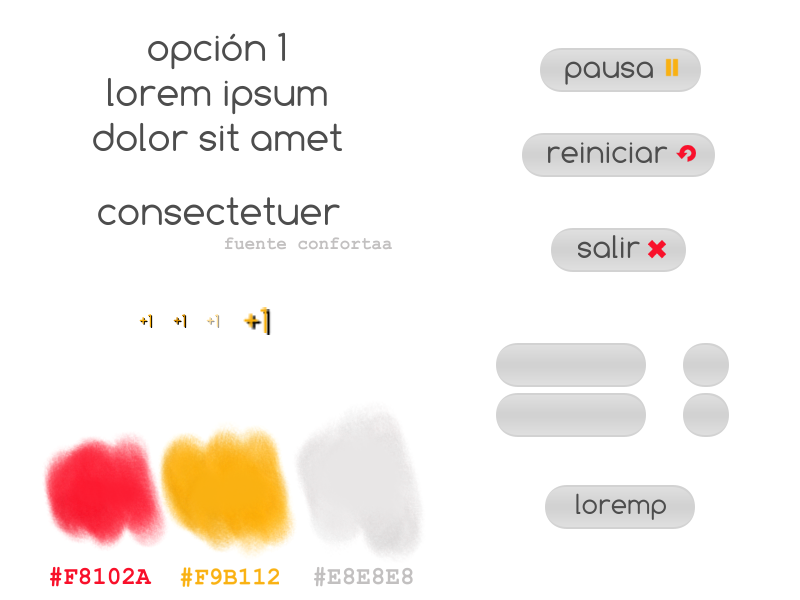
\includegraphics[scale=0.5]{ui.png}
  \end{center}
  \caption{Diferentes elementos utilizados en la interfaz}
\end{figure}

\subsection{Documentación del código}

Por otro lado, para gestionar toda la documentación del proyecto se decidió utilizar las siguientes herramientas:
\begin{itemize}
    \item \LaTeX\ para escribir la memoria, ya que es una forma robusta y fiable de escribir una memoria para
            un Proyecto Fin de Carrera, descartándose otras posibles opciones por no ser adecuadas para la escritura
            de un documento de estas características. Para facilitar la compilación dispone de la herramienta
            GNU Make~\cite{pdf:make}.
    \item Doxygen para la documentación del código fuente, porque además de documentar de manera sencilla y fácil
            de leer el mismo código fuente, genera una documentación en diferentes formatos. Además,
        \begin{itemize}
            \item Doxygen funciona con lenguajes como C++, C, Java, Objective-C, Python, Fortran, VHDL, PHP o C\#
                    (entre otros), por lo que se puede acomodar a nuestras necesidades. Incluso existe una
                    herramienta llamada \textbf{Doxypy} que nos permite reutilizar los comentarios \emph{tipo Python}
                    y adaptarlos a Doxygen, con lo cual ahorramos trabajo y cumplimos con la normativa
                    de código Python.
        \end{itemize}
\end{itemize}

\subsection{Sistema de control de versiones}

El código del proyecto Dominous, está alojado por completo dentro del sistema que proporciona Rediris, que básicamente
consiste en un entorno completo basado en Subversion -- SVN. \\ 

Subversion permite llevar un control exahustivo de todos los ficheros e iteraciones de código que se realizan en él,
permitiendo volver a versiones anteriores de código, comprobar diferencias entre versiones o ficheros y cualquier otra
operación propia de un sistema de control de versiones. \\

Se evaluaron otros sistemas de control de versiones distribuidos como GIT, Bazaar o Mercurial, pero se desecharon
básicamente porque, por un lado, este proyecto cuenta únicamente con un desarrollador, y multitud de ventajas que
ofrecen los sistemas de control de versiones distribuidos dejan de tener sentido, si tenemos en cuenta esta circunstancia
del proyecto, y por otro lado la integración de SVN con Rediris (con las ventajas de visualización de código y versiones
que ofrece ViewCVS) decantaron la decisión sobre el lado de SVN.

\section{Interfaz gráfica}

Tomando los resultados obtenidos en la fase de análisis es necesario diseñar una interfaz gráfica amigable
para el usuario y desde la cual se pueda interactuar con la aplicación. Para el diseño de las interfaces
se intentará en todo momento que sean usables además de intentar conseguir que el usuario no pueda
introducir datos erróneas para que no produzca comportamientos anómalos. \\

\begin{figure}[h]
  \label{fig:pantallas_interfaz}
  \begin{center}
    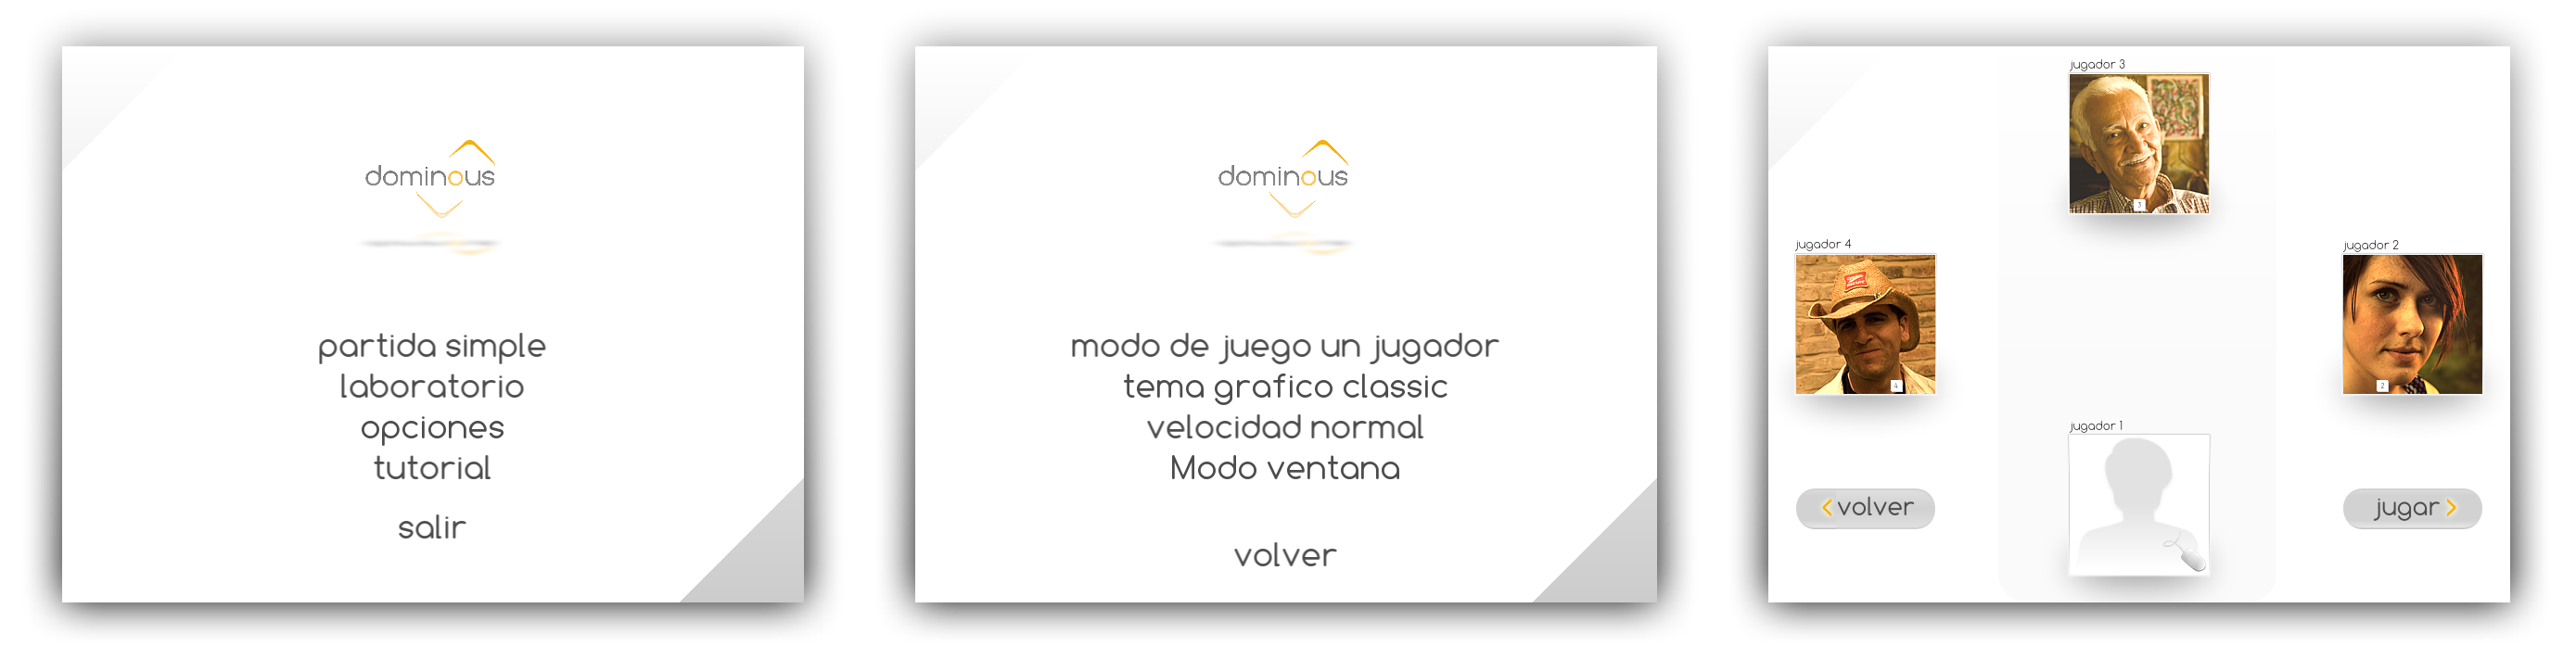
\includegraphics[scale=0.25]{interfaz.png}
  \end{center}
  \caption{Varias pantallas con la interfaz de Dominous}
\end{figure}

\subsection{Diagrama de interacción entre interfaces gráficas}

En el siguiente diagrama~\ref{fig:diagramainteraccioninterfaces} podemos observar la interacción entre
las distintas interfaces gráficas desarrolladas para la aplicación. \\

\begin{figure}[h]
  \label{fig:diagramainteraccioninterfaces}
  \begin{center}
    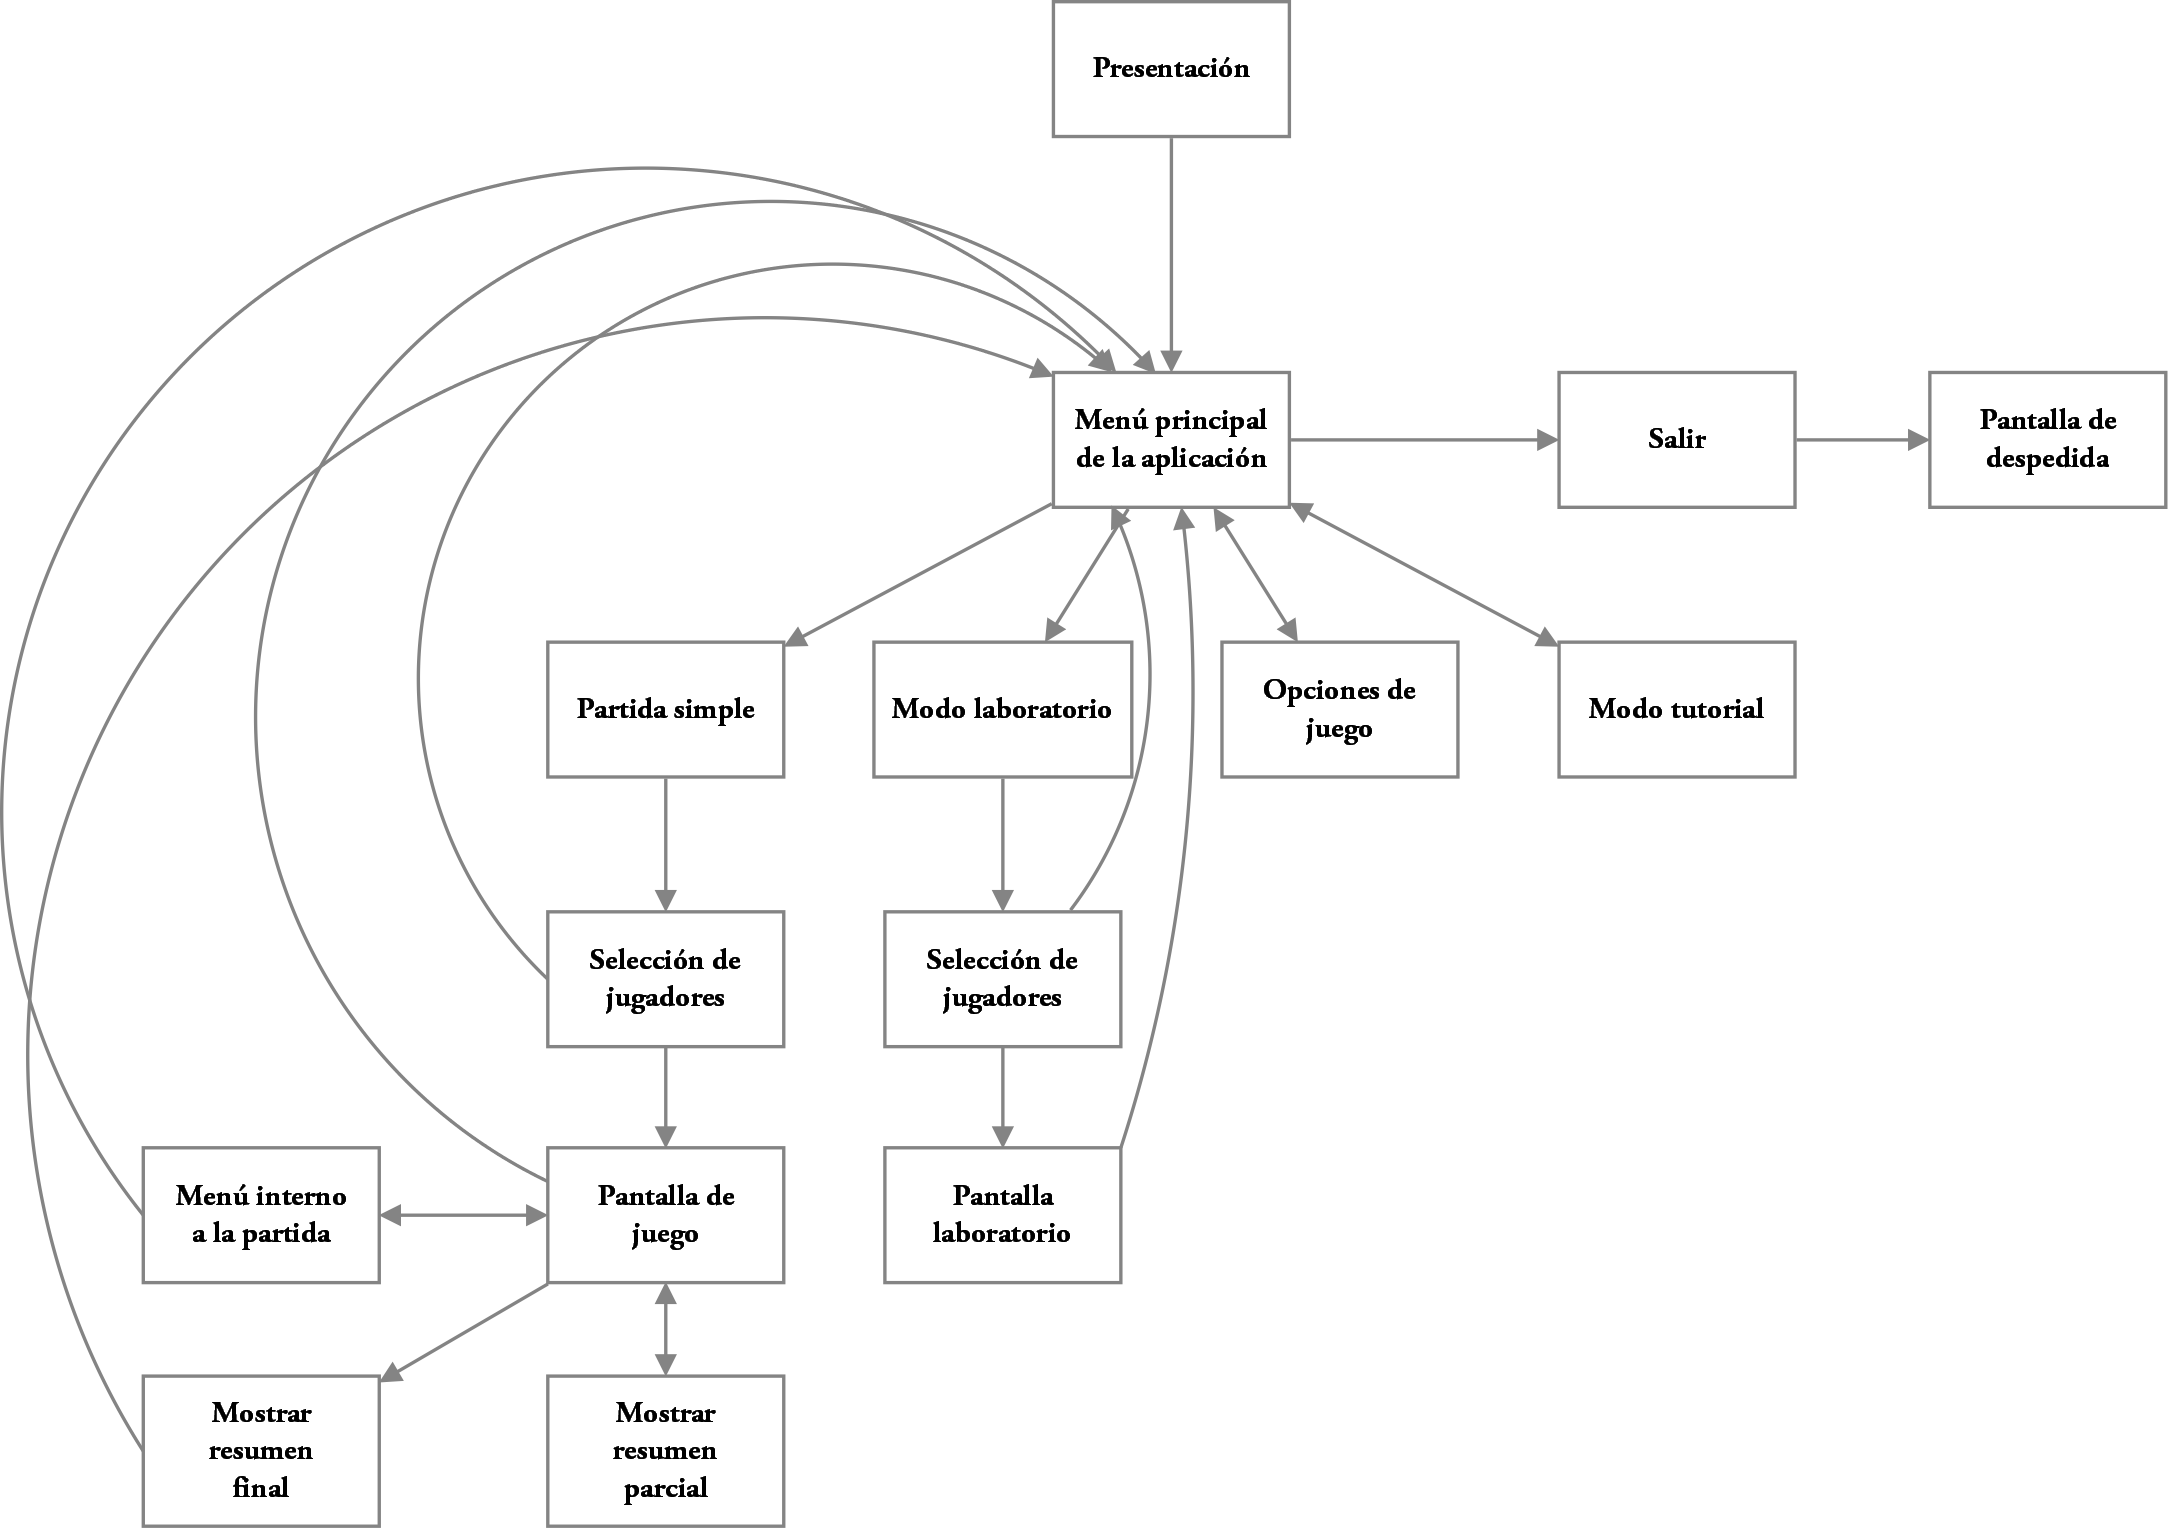
\includegraphics[scale=0.15]{diagrama_interfaces.png}
  \end{center}
  \caption{Diagrama de interacción entre interfaces}
\end{figure}

\section{Diagrama Entidad -- Relación}

La aplicación \textbf{Dominous} realiza un almacenamiento limitado de información, por lo que no se estima necesario
realizar un diagrama Entidad -- Relación con este fin.

\section{Diagrama de clases de diseño}

A continuación se muestra el diagrama de clases de diseño para \textbf{Dominous}.

\begin{figure}[h]
  \label{diagrama_clases_diseno}
  \begin{center}
    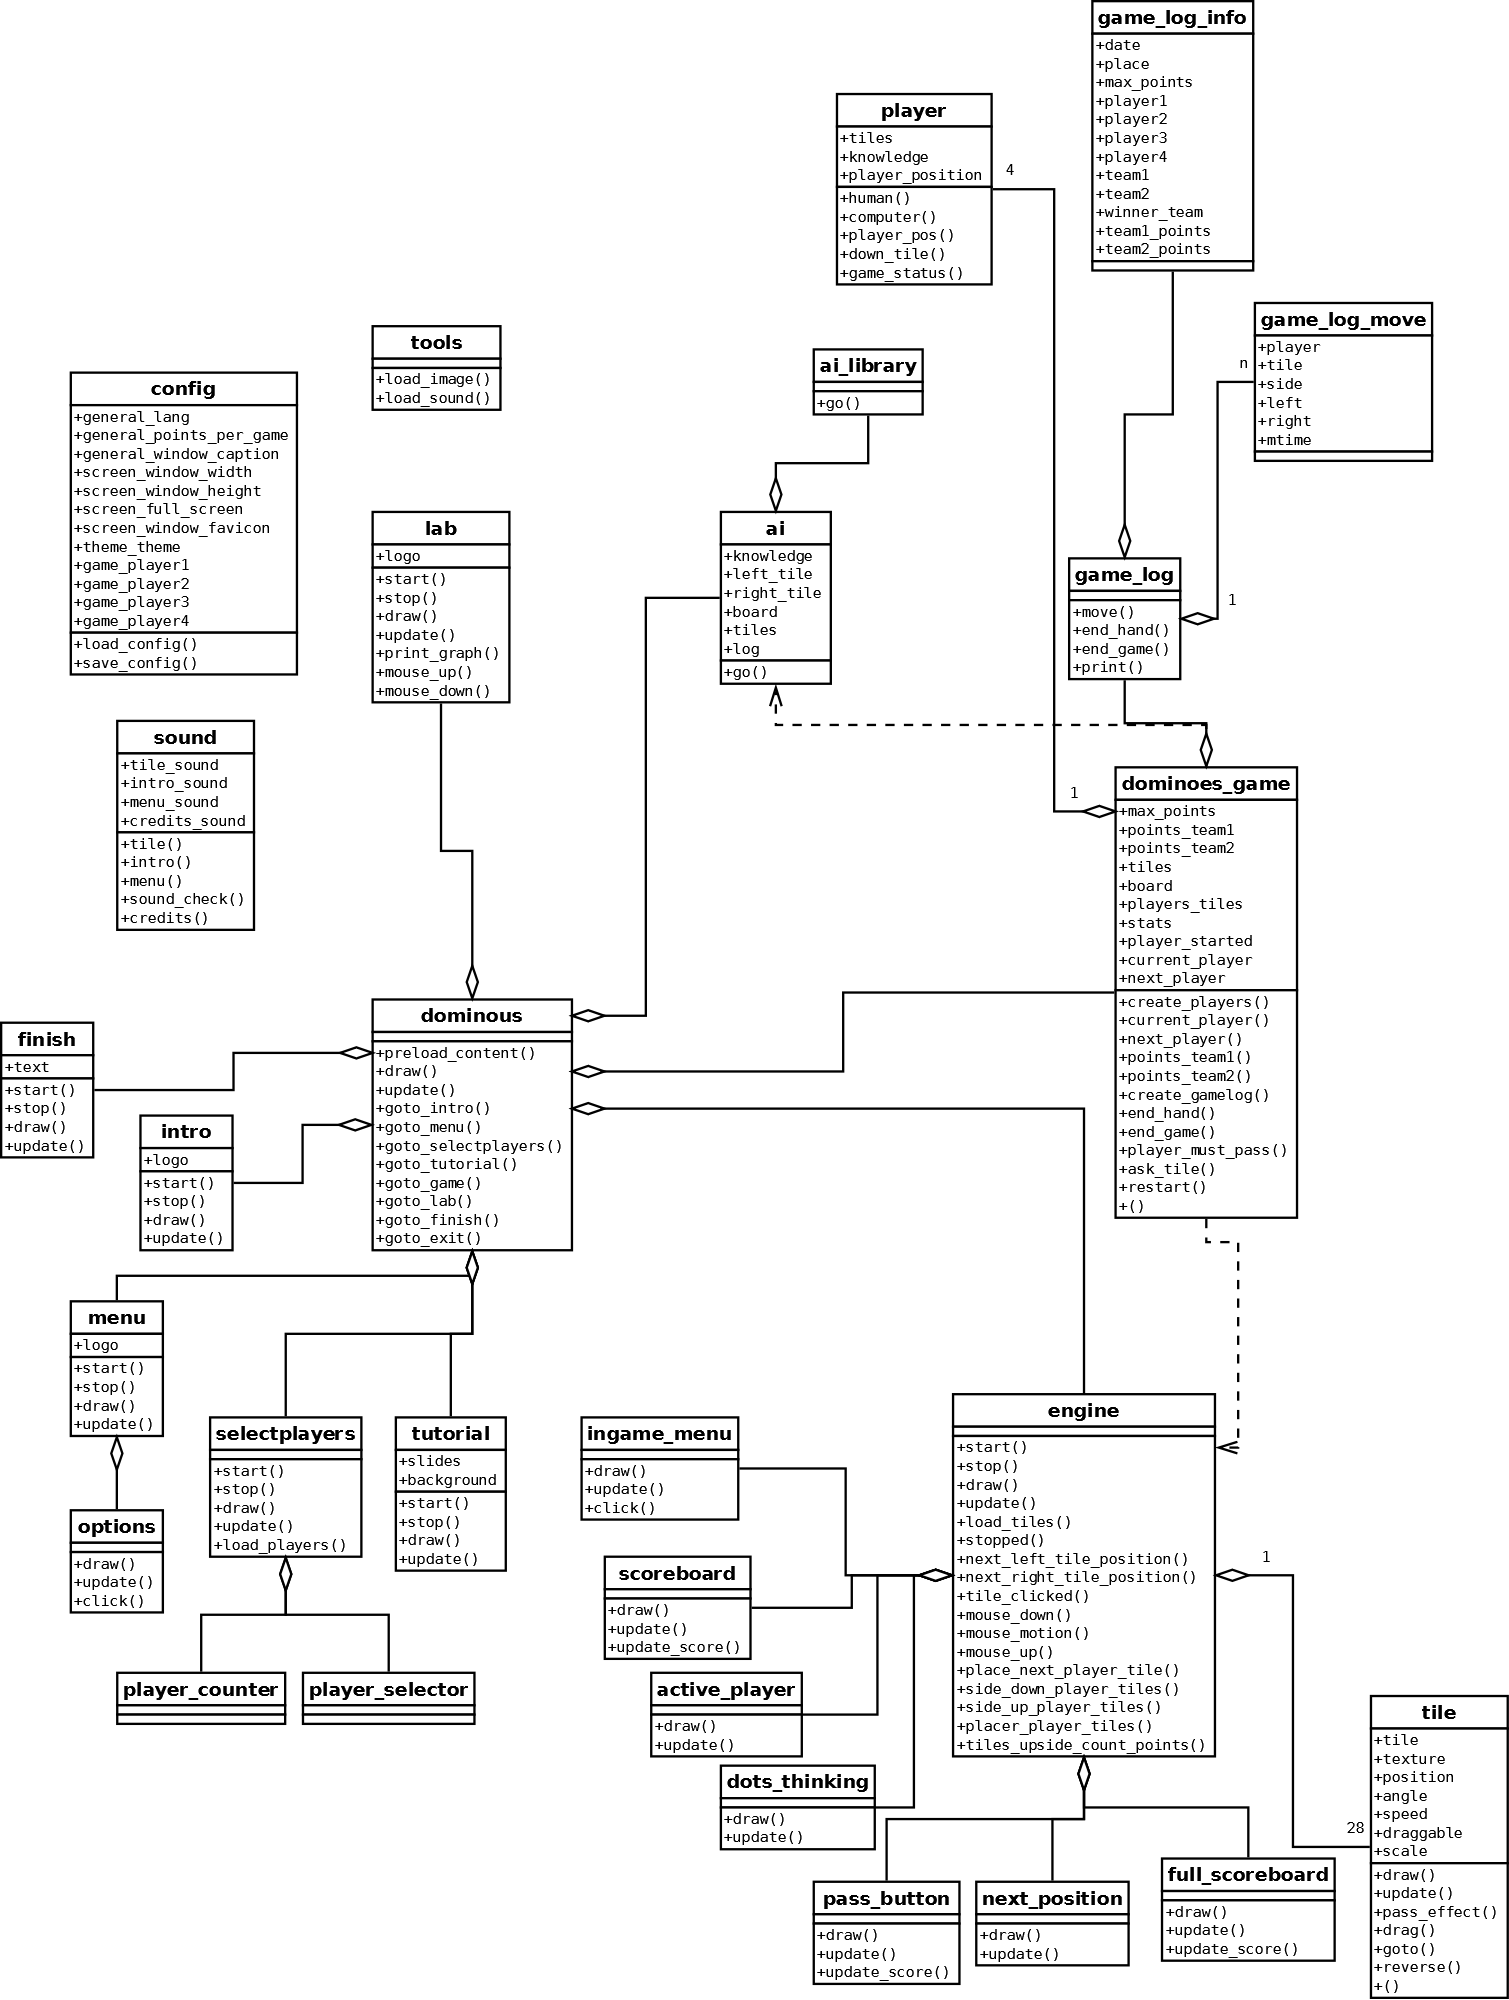
\includegraphics[scale=0.23]{diagrama_clases_diseno.png}
  \end{center}
  \caption{Diagrama de diseño del sistema}
\end{figure}


\section{Análisis de las principales clases de la aplicación}

En este apartado realizaremos un repaso a las principales clases que intervienen en el diseño de \textbf{Dominous},
definiendo los métodos y atributos que se requieren para el correcto desarrollo de la aplicación y comentando
todos los apartados cuya funcionalidad merezca ser destacada.

\subsection{Clase dominous}

La clase dominous genera el objeto principal que soporta el peso principal de toda la aplicación. Al inicio de la
ejecución se crea un objeto de esta clase; este objeto va creando --- según las necesidades del flujo que tome
la ejecución de la misma --- los diferentes objetos, controlando y dando paso a la interfaz activa, llamando a
las principales funciones y permitiendo la captura de los eventos de entrada. \\

Al igual que la gran mayoría de videojuegos, para el desarrollo de Dominous se han utilizado dos métodos principales
que permiten controlar la aplicación en tiempo real. Estos dos métodos son:
\begin{description}
    \item[draw] El primer método se encarga de dibujar en pantalla todos los elementos de la interfaz. El funcionamiento
        básico es recorrer todos los objetos activos y pintarlos según la posición, rotación y escala que tengan en
        ese preciso momento. 
    \item[update] El segundo método se ocupa de realizar los cálculos para el movimiento de los elementos gráficos. 
        En cada iteración cambiará el estado de los objetos activos, modificando la imagen o los valores posición,
        rotación y/o escala, estudiando las posibles colisiones, eventos y cualquier otra circunstancia que cambie
        el estado de la aplicación, para que en el siguiente ciclo se dibujen los elementos en su posición correcta.
\end{description}

Una vez que este objeto principal toma el control de la aplicación, su función es llamar a los métodos \comando{draw}
y \comando{update} del objeto encargado de la interfaz que estemos mostrando actualmente, de forma alternativa. \\

Este juego de llamadas a ambos métodos se realizará hasta un máximo de 60 veces por segundo, dependiendo del rendimiento
que se obtenga de los recursos del sistema. De esta forma conseguiremos un máximo de 60 frames o cuadros por segundo,
que serán los encargados de generar la sensación de movimiento. \\

Como vemos, el objeto de la clase dominous no realiza ningún dibujado en pantalla ni cálculos, sino que su único
cometido es redireccionar el flujo de la aplicación al objeto correspondiente.

\subsection{Clase dominoes\_game}

La labor de esta clase es llevar el control de una partida completa de dominó, siguiendo las reglas del \textbf{dominó
internacional}. Dependiendo de la configuración de la partida, creará los jugadores según la selección que se haya
realizado en la pantalla de selección de personajes y comenzará con el bucle principal: \\

Repartirá las fichas entre los diferentes participantes del juego e irá pidiendo fichas a los jugadores de forma
consecutiva, hasta que se de alguna circunstancia de finalización de la mano. \\

Este bucle se repetirá hasta que alguno de los dos equipos alcance o supere los 200 puntos, momento en el cual la partida
se dará por finalizada. \\

Esta clase también mantendrá activo y actualizado un fichero de log con toda la información generada en la partida. Esta
información se utilizará más tarde en el apartado de inteligencia artificial, y almacenará los datos utilizando
la siguiente estructura: \\

Por un lado tenemos la información global de la partida: 

\begin{description}
    \item[date] Fecha de desarrollo de la partida.
    \item[place] Lugar donde tuvo lugar la partida.
    \item[max\_points] Límite superior de puntos necesarios para ganar el encuentro. Como se utilizan las reglas del
        \textbf{dominó internacional}, esta cota estará situada en los doscientos puntos.
    \item[player1] Datos del jugador 1.
    \item[player2] Datos del jugador 2.
    \item[player3] Datos del jugador 3.
    \item[player4] Datos del jugador 4.
    \item[team1] Pareja que forma el equipo 1.
    \item[team2] Pareja que forma el equipo 2.
    \item[points\_team1] Puntos actuales que tiene el equipo 1.
    \item[points\_team2] Puntos actuales que tiene el equipo 2.
    \item[winner\_team] Pareja que finalmente ha sido ganadora de la partida.
\end{description}

Y por otro lado tenemos información relativa a la mano que se está desarrollando actualmente. Esta información se repite
por cada movimiento que se realice en la partida, y se agrupa por manos:

\begin{description}
    \item[player] Jugador que ha realizado el movimiento.
    \item[tile] Ficha que ha colocado.
    \item[side] Lado del tablero por donde ha colocado la ficha.
    \item[left] Cifra, del cero al siete, que se tiene como resultante del movimiento por el lado izquierdo del tablero.
    \item[right] Cifra, del cero al siete, que se tiene como resultante del movimiento por el lado derecho del tablero.
    \item[mtime] Tiempo (en segundos) que ha estado pensando el jugador antes de colocar la ficha.
\end{description}


\section{Sistemas expertos}

En este apartado de la memoria requiere de una especial explicación, ya que a la hora de realizar un videojuego de
dominó goza de gran importancia los diferentes sistemas expertos que participarán en la partida. Estos sistemas expertos,
como bien su nombre indica, simulan el comportamiento de un ser humano experto en una materia, en este caso del juego
de dominó, y su realismo debe hacer sentir al jugador humano que está desempeñando una partida real contra jugadores
también humanos. \\

Enfrentarse a una simulación de inteligencia artificial es una de las empresas más difíciles y complicadas pero a la
vez placenteras y satisfactorias de abarcar en un proyecto de Ingeniería del Software. Los seres humanos utilizan
multitud de métodos y herramientas para razonar y obtener soluciones a problemas concretos, y en muchas ocasiones
este tipo de comportamientos son imposibles de simular, bien por la complejidad computacional que supone, bien por
desconocimiento del funcionamiento exacto que sigue el cerebro para obtener esa solución, o bien por limitaciones de
recursos, ya sea de disco, tiempo de desarrollo o metodologías que simulen ese comportamiento. \\

Por otro lado, aunque el público neófito en la materia pueda suponer que el dominó es un juego de suerte, con un
abanico muy corto de opciones de juego o con una libertad de movimientos muy limitada, nada más lejos de la realidad. \\

El dominó es un juego muy profundo, con normas, técnicas y muchas dosis de psicología, un deporte que obliga al
jugador a estar concentrado al cien por cien durante todo el desarrollo del juego, y un arte con una curva de
aprendizaje poco escarpada, que permite que jugadores nóveles puedan adentrarse en el juego, pero que presenta
mucha complicación convertirse en un gran jugador de dominó. \\

Y, si estas razones que explican la complejidad del mismo no fueran suficientes, no hay más que echarle un vistazo
a los torneos locales o de ámbitos más abiertos para descubrir que las parejas de grandes jugadores sabios y con
una gran compenetración son los que suelen ganar, descartando de forma tajante la posibilidad de que sea la suerte
la que empuje la balanza de la partida hacia un equipo u otro. \\

A la hora de afrontar este problema, el primer paso fue empaparse de cultura y conocimiento sobre el dominó. Las
principales herramientas que se utilizaron fueron:

\begin{description}
    \item[El Libro del dominó] de Benito Ruipérez \cite{mora90}, un libro ameno y profundo sobre el mundo del dominó,
        con multitud de partidas explicadas movimiento a movimiento, trucos, ejemplos, técnicas básicas y avanzadas y
        mucha información.
    \item[Don Manuel Palomo Fernández de Bobadilla] -- jugador amateur de dominó y participante en torneos durante más de cuarenta
        años, con un gran conocimiento de técnicas y métodos de juego, mucha experiencia y una gran facilidad para
        comunicar toda esa sabiduría y conocimiento.
\end{description}

Después de profundizar en el mundo del dominó, y tener cierto conocimiento sobre el mismo --- aunque nada comparado
con el que pueden tener jugadores más experimentados de este juego --- podemos intentar definir las pautas sobre
las que va a llevarse a cabo la simulación del sistema experto de dominó. \\

Lo primero que observamos es que la estrategia que siga cada jugador depende enteramente del rol que desempeñe el mismo.
Como vimos en el capítulo ~\ref{juegoporparejas} es importante definir una estrategia personalizada para cada jugador,
dependiendo del lugar respecto al jugador mano.
